\documentclass[12pt,letterpaper]{article}

\usepackage[letterpaper, margin=1in]{geometry}
\usepackage[utf8]{inputenc} % OJO!!!  => MANTENER ESTA LINEA PARA FACIL CONVERSION A WORD EN EL FUTURO ...
% \usepackage[spanish]{babel}
\usepackage{graphicx} 
\usepackage{array}
\usepackage{tabularx}
\usepackage{amssymb, amsmath}

% Paquetes extras ... 
\usepackage{subfigure}
\usepackage{color}
\definecolor{mygreen}{RGB}{28,172,0} % color values Red, Green, Blue
\definecolor{mylilas}{RGB}{170,55,241}

\usepackage{hyperref}
\usepackage{enumitem}

\usepackage{amsmath,amsfonts,amssymb,amsthm,cancel,icomma,nicefrac,mathrsfs,
            eurosym,verbatim,environ,ifthen,ifdraft,pdfpages,float,booktabs}
\allowdisplaybreaks[1] 

\usepackage{color}
\definecolor{lstgrey}{rgb}{0.95,0.95,0.95}
\usepackage{listings}
\lstset{language=Matlab,
       backgroundcolor=\color{lstgrey},
       frame=single,
       basicstyle=\footnotesize\ttfamily,
       captionpos=b,
       tabsize=2,
  }

\lstset{language=Matlab,%
  %basicstyle=\color{red},
  breaklines=true,%
  morekeywords={matlab2tikz},
  keywordstyle=\color{blue},%
  morekeywords=[2]{1}, keywordstyle=[2]{\color{black}},
  identifierstyle=\color{black},%
  stringstyle=\color{mylilas},
  commentstyle=\color{mygreen},%
  showstringspaces=false,%without this there will be a symbol in the places where there is a space
  numbers=left,%
  numberstyle={\tiny \color{black}},% size of the numbers
  numbersep=9pt, % this defines how far the numbers are from the text
  emph=[1]{for,end,break},emphstyle=[1]\color{red}, %some words to emphasise
  %emph=[2]{word1,word2}, emphstyle=[2]{style},    
}


\title{Homework 4 - RIDF Analysis}
\author{Jose Eduardo Laruta Espejo \\ Facultad de Ingeniería - Universidad Mayor de San Andrés}
\begin{document}
\maketitle

\section{Tracker Model}
In this case, we need to use the piece-wise linear characteristic of the ideal limiter, from slide 20:

\begin{align}
    \phi(v)     &= \left\{\begin{array}{ll}
                            v               &  |v| \leq \delta \\
                            \delta sign(v) &  |v| > \delta
                        \end{array}
                    \right. \\
    \hat{\phi}  &= \sigma \left[ G(\frac{\delta + m}{\sigma}) - G(\frac{\delta - m}{\sigma}) - 1\right] - m \\
    N_{\phi}    &= F(\frac{\delta + m}{\sigma}) - F(\frac{\delta - m}{\sigma}) - 1 
\end{align}

For the Matlab implementation is important to point out that the functions $F$ and $G$ 
have been implemented using anonymous functions inside de model function (lines 13 and 14). This is 
for the code being more readable.

Another global parameter was added corresponding the value of $\delta$ for the limit of 
the saturation model. In this case, for simulating a linear case we use the \texttt{Kant} global variable
when it is equal to zero, then the values of $\hat{\phi}$ and $N_{\phi}$ are forced 
to te corresponding values for the linear model (lines 18-20).

\lstinputlisting[label=lst:model]{../matlab/tracker_ridf_erf.m}

\section{RIDF Analysis}
Using the same initial conditions and parameters given for the problem in the slides, we 
can simulate the three models: linear, RIDF for cubic nonlinearity and RIDF for piece-wise 
linear saturation. The results can be seen in Fig  

%%%% Figura 1 %%%%%%
\begin{figure}[!h] 
    \centering
    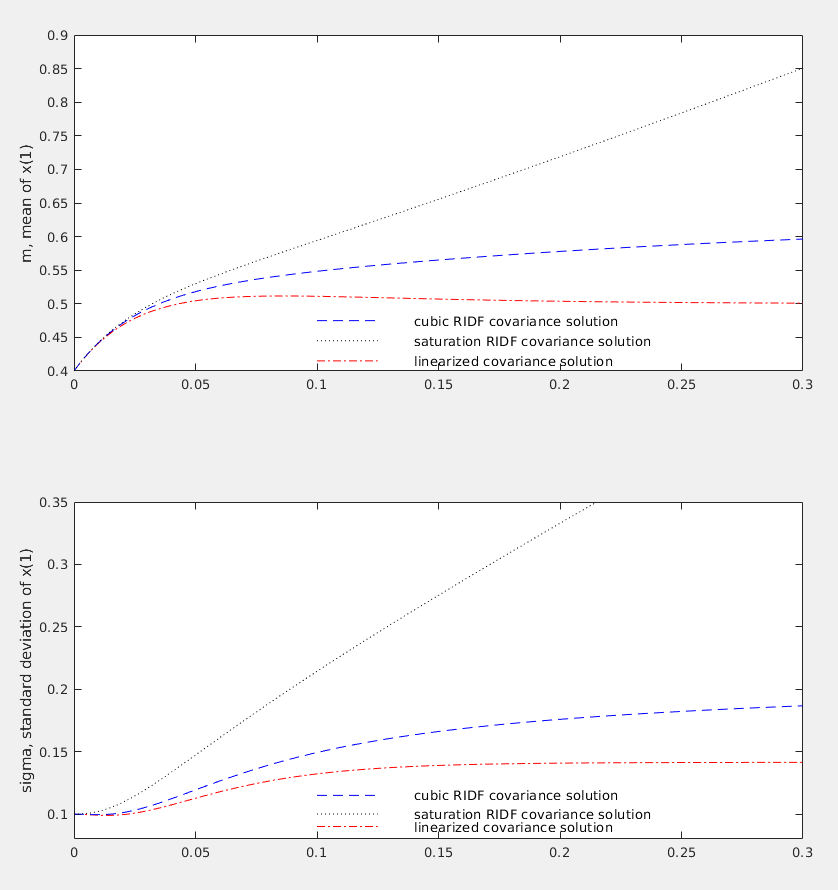
\includegraphics[width=\textwidth]{../matlab/img/simu2.png}
    \caption{Covariance Analysis of the three models}
    \label{fig:simu}
    \end{figure}
  
\end{document}